\chapter{Disain}
\label{chap:disain}

\section{Disain Antarmuka}
\label{sec:disainantarmuka}

\hspace{0,5cm}Pada sub-bab ini akan dibahas mengenai disain antar muka aplikasi \textit{mobile} dan \textit{website}.

\subsection{Disain Aplikasi \textit{Mobile}}
\label{subsec:disainaplikasimobile}

\hspace{0,5cm}Pada aplikasi \textit{mobile} terdapat beberapa halaman utama pendukung fitur, yakni:
\begin{enumerate}
	\item Halaman \textit{login}
	\item	Halaman pendaftaran
	\item Halaman pengisian profil rumah tangga
	\item Halaman \textit{dashboard}
	\item Halaman penambahan anggota
	\item Halaman anggota keluarga
	\item Halaman pengolahan kategori transaksi
	\item Halaman penambahan kategori
	\item Halaman transfer
	\item Halaman penambahan pemasukan
	\item Halaman penambahan pengeluaran
	\item Halaman pemilihan laporan
	\item Halaman laporan
\end{enumerate}


\begin{figure}
\centering
\resizebox{\textwidth}{!}{
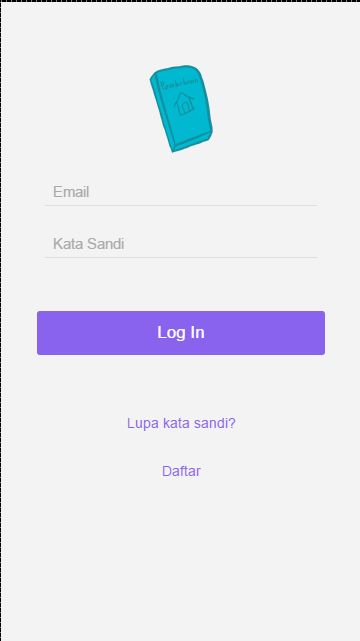
\includegraphics[scale=0.01]{Gambar/design-app/login}
}
\caption[Tampilan \textit{login}]{Tampilan \textit{login}} 
\label{fig:design_app_login}
\end{figure}


\begin{figure}
\centering
\resizebox{\textwidth}{!}{
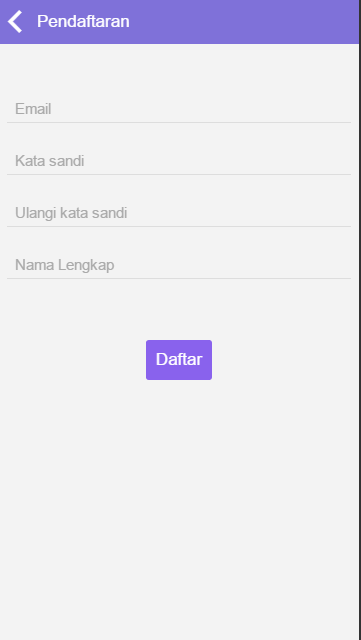
\includegraphics[scale=0.01]{Gambar/design-app/register}
}
\caption[Tampilan pendaftaran]{Tampilan pendaftaran} 
\label{fig:design_app_pendaftaran}
\end{figure}

\begin{figure}
\centering
\resizebox{\textwidth}{!}{
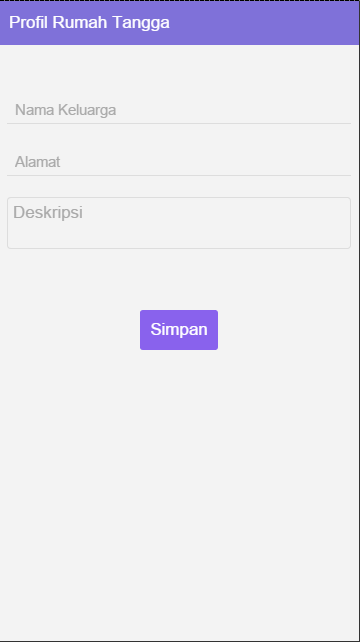
\includegraphics[scale=0.01]{Gambar/design-app/profil_awal}
}
\caption[Tampilan pengisian profil rumah tangga]{Tampilan pengisian profil rumah tangga} 
\label{fig:design_app_profil awal}
\end{figure}

\begin{figure}
\centering
\resizebox{\textwidth}{!}{
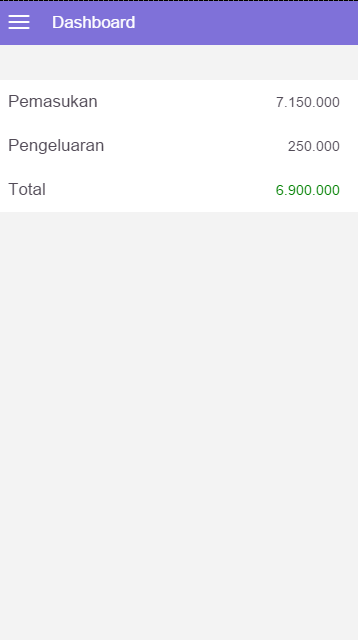
\includegraphics[scale=0.01]{Gambar/design-app/dashboard}
}
\caption[Tampilan \textit{dashboard}]{Tampilan \textit{dashboard}} 
\label{fig:design_app_dashboard}
\end{figure}

\begin{figure}
\centering
\resizebox{\textwidth}{!}{
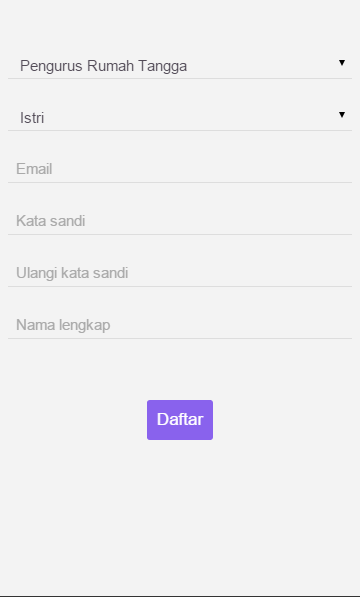
\includegraphics[scale=0.01]{Gambar/design-app/penambahan_anggota}
}
\caption[Tampilan penambahan anggota]{Tampilan penambahan anggota} 
\label{fig:design_app_penambahan_anggota}
\end{figure}

\begin{figure}
\centering
\resizebox{\textwidth}{!}{
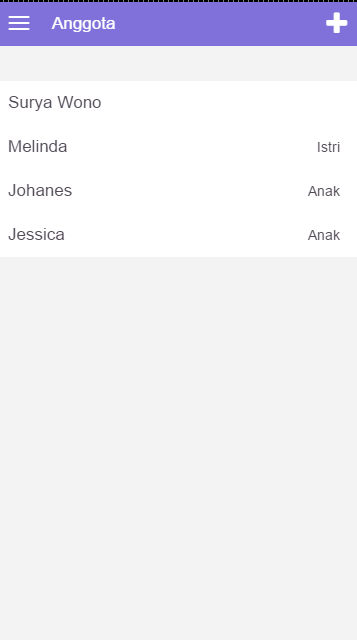
\includegraphics[scale=0.01]{Gambar/design-app/anggota_keluarga}
}
\caption[Tampilan anggota keluarga]{Tampilan anggota keluarga} 
\label{fig:design_app_anggota_keluarga}
\end{figure}

\begin{figure}
\centering
\resizebox{\textwidth}{!}{
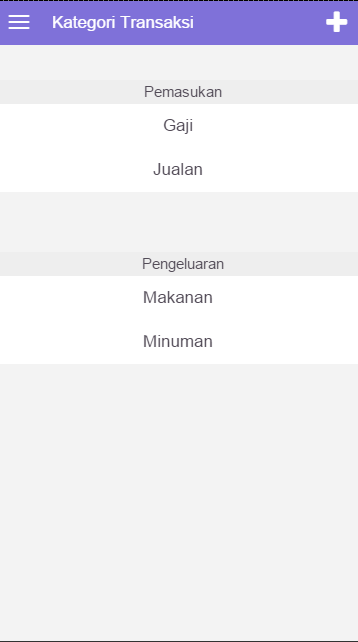
\includegraphics[scale=0.01]{Gambar/design-app/kategori_transaksi}
}
\caption[Tampilan pengolahan kategori transaksi]{Tampilan pengolahan kategori transaksi} 
\label{fig:design_app_kategori_transaksi}
\end{figure}

\begin{figure}
\centering
\resizebox{\textwidth}{!}{
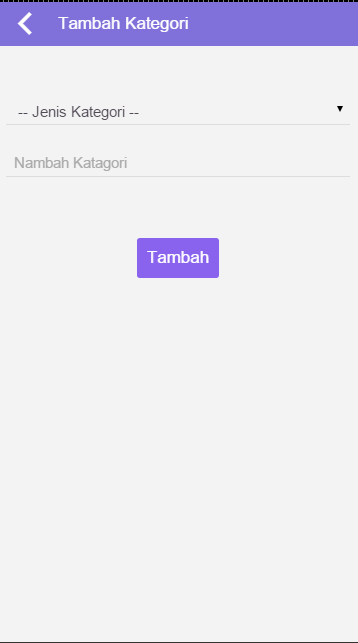
\includegraphics[scale=0.01]{Gambar/design-app/penambahan_kategori}
}
\caption[Tampilan penambahan kategori]{Tampilan penambahan kategori} 
\label{fig:design_app_penambahan_kategori}
\end{figure}

\begin{figure}
\centering
\resizebox{\textwidth}{!}{
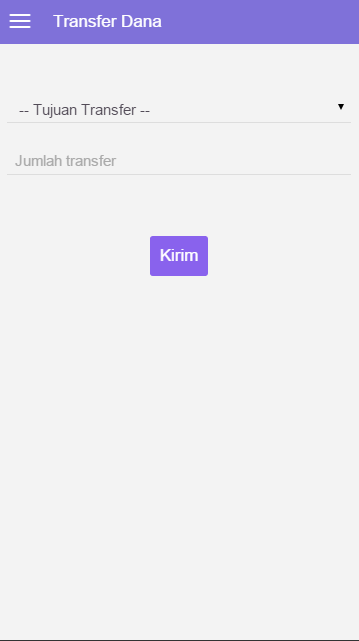
\includegraphics[scale=0.01]{Gambar/design-app/transfer}
}
\caption[Tampilan transfer]{Tampilan transfer} 
\label{fig:design_app_transfer}
\end{figure}

\begin{figure}
\centering
\resizebox{\textwidth}{!}{
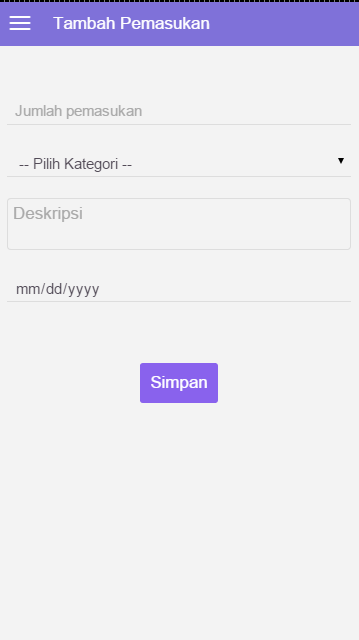
\includegraphics[scale=0.01]{Gambar/design-app/penambahan_pemasukan}
}
\caption[Tampilan penambahan pemasukan]{Tampilan penambahan pemasukan} 
\label{fig:design_app_penambahan_pemasukan}
\end{figure}

\begin{figure}
\centering
\resizebox{\textwidth}{!}{
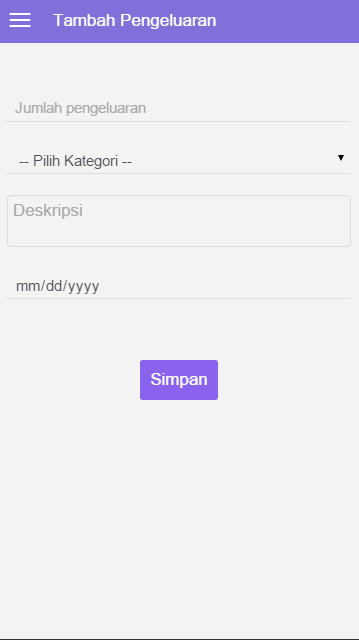
\includegraphics[scale=0.01]{Gambar/design-app/penambahan_pengeluaran}
}
\caption[Tampilan penambahan pengeluaran]{Tampilan penambahan pengeluaran} 
\label{fig:design_app_penambahan_pengeluaran}
\end{figure}

\begin{figure}
\centering
\resizebox{\textwidth}{!}{
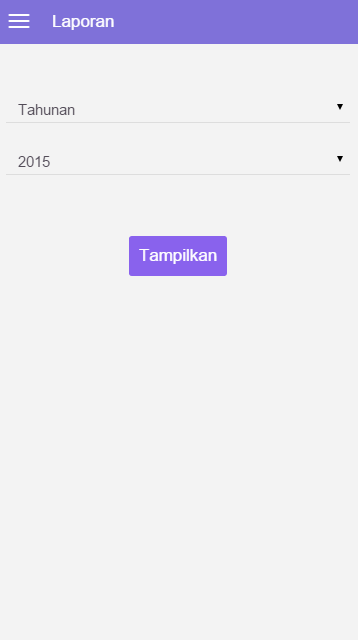
\includegraphics[scale=0.01]{Gambar/design-app/pemilihan_laporan}
}
\caption[Tampilan pemilihan laporan]{Tampilan pemilihan laporan} 
\label{fig:design_app_pemilihan_laporan}
\end{figure}

\subsection{Disain Apliasi \textit{Website}}
\label{subsec:disainaplikasiwebsite}

\hspace{0,5cm}Pada aplikasi \textit{website} terdapat beberapa halaman utama pendukung fitur, yakni;
\begin{enumerate}
	\item Halaman \textit{login}
	\item Halaman \textit{dashboard}
	\item Halaman daftar rumah tangga
	\item Halaman pengololahan kategori transaksi
	\item Halaman pelaporan
\end{enumerate}

\begin{figure}
\centering
\resizebox{\textwidth}{!}{
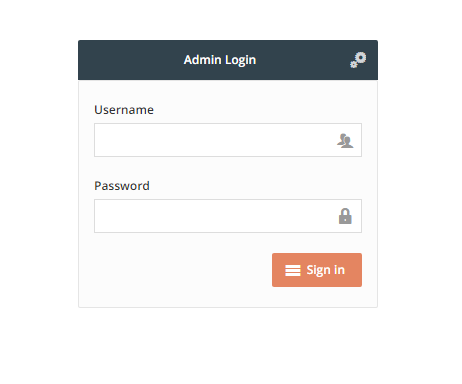
\includegraphics[scale=0.01]{Gambar/design-web/login}
}
\caption[Tampilan login]{Tampilan login} 
\label{fig:design_web_login}
\end{figure}

\begin{figure}
\centering
\resizebox{\textwidth}{!}{
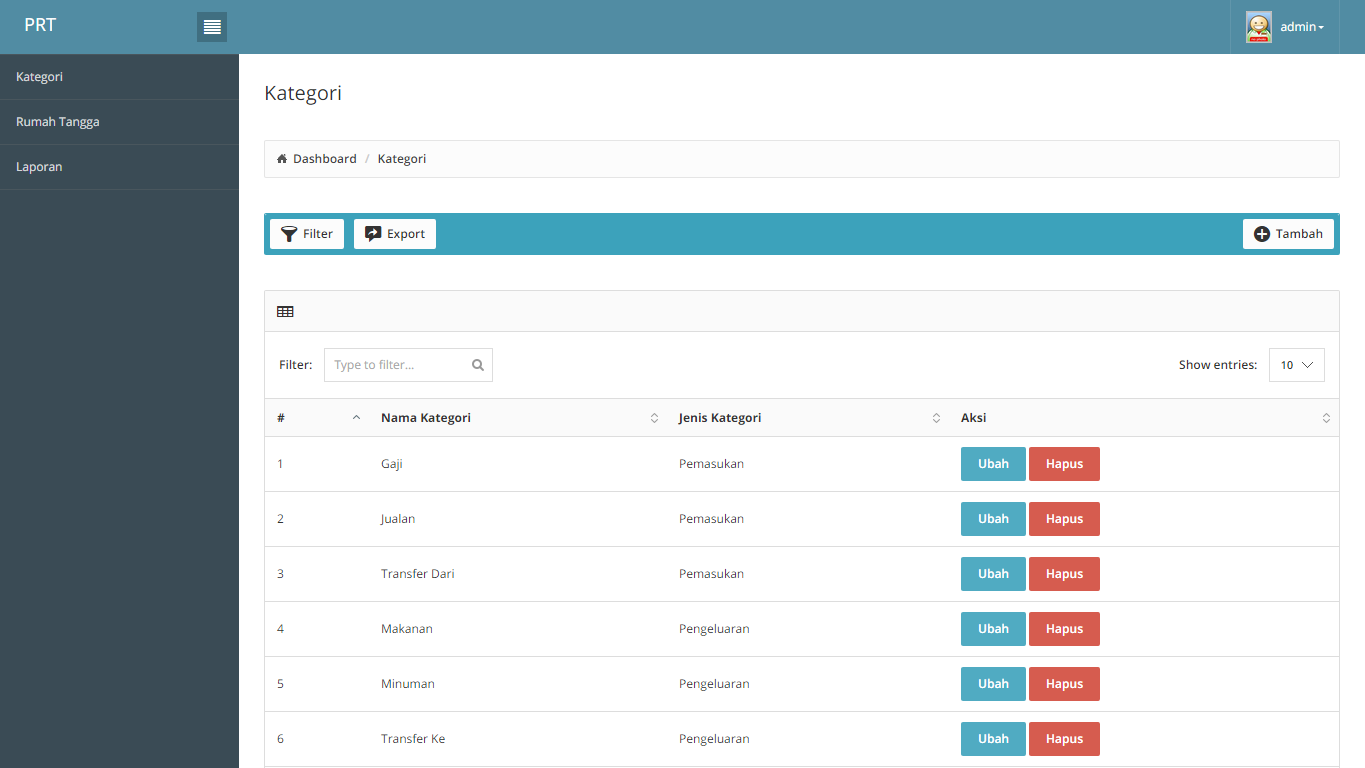
\includegraphics[scale=0.01]{Gambar/design-web/index_kategori}
}
\caption[Tampilan halaman kategori]{Tampilan halaman kategori} 
\label{fig:design_web_index_kategori}
\end{figure}

\begin{figure}
\centering
\resizebox{\textwidth}{!}{
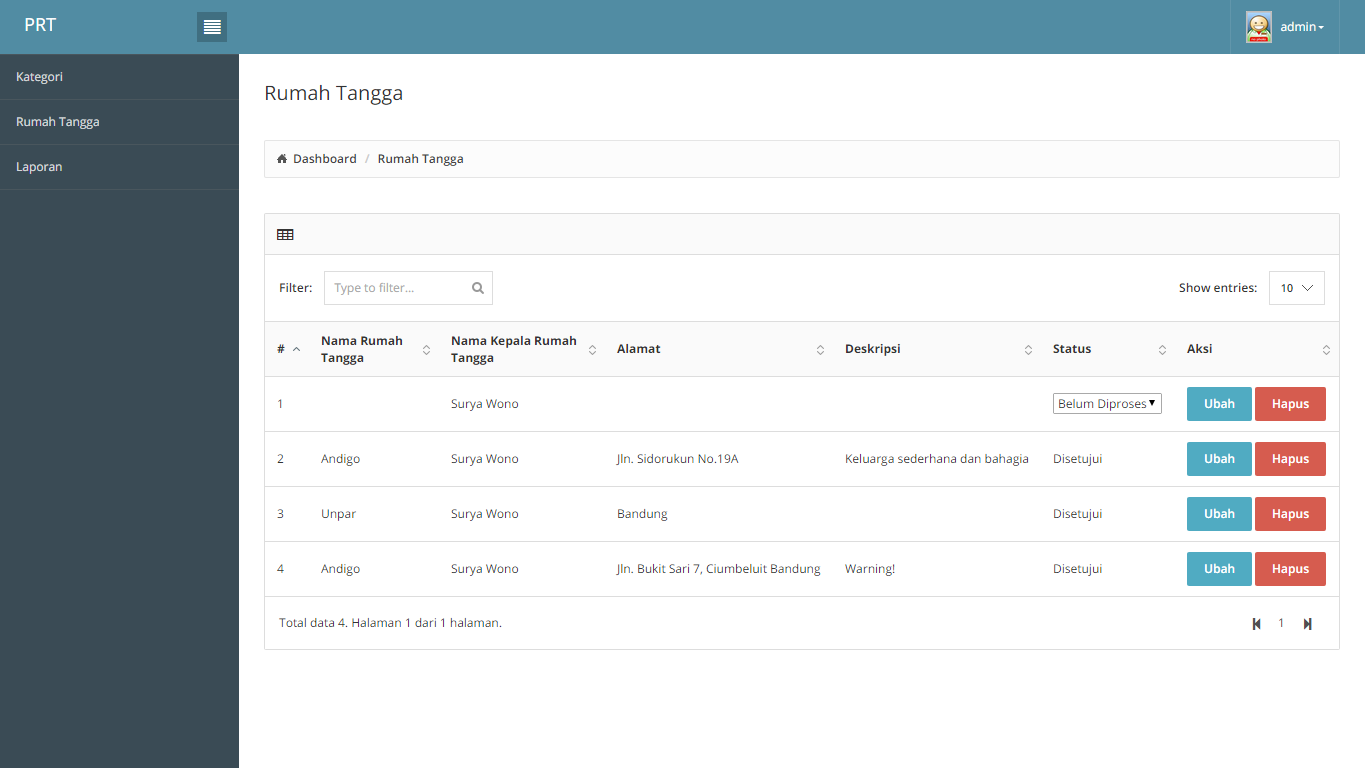
\includegraphics[scale=0.01]{Gambar/design-web/index_rumah_tangga}
}
\caption[Tampilan halaman rumah tangga]{Tampilan halaman rumah tangga} 
\label{fig:design_web_index_rumah_tangga}
\end{figure}

\section{Disain Basis Data}
\label{sec:disainbasisdata}

\section{Disain Layanan}
\label{sec:disainlayanan}



